\chapter{Navigation}\label{cha:navigation}

In diesem Kapitel wird die ''moving map'' beschreiben, welche einen elementaren Bestandteil von \xc zur Navigation darstellt und heute selbstverständlich ist. 
Weiterhin werden hier die entsprechenden Elemente beschrieben, welche auf der Karte eingeblendet sind um die Navigation so schnell und einfach wie möglich zu machen.

\section{Elemente der Kartenanzeige}

\begin{maxipage}\centering
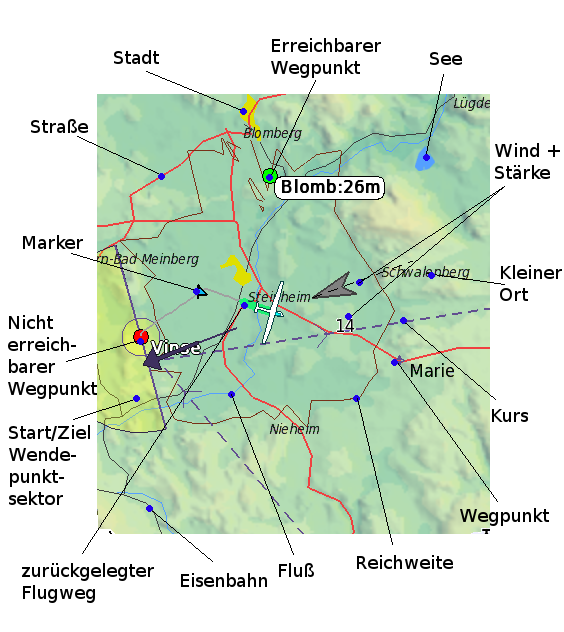
\includegraphics[angle=0,width=0.55\linewidth,keepaspectratio='true']{figures/fig-map.png}
\end{maxipage}

Die moving-map zeigt folgende Bestandteile:

\begin{enumerate}[itemsep=-0.25ex]
  \item Das Segelflugzeug Symbol
  \item Die Wegpunkte
  \item Die aktive Flugaufgabe (''task'')
  \item Den Kurs zum gewählten Wegpunkt (''bearing'')
     (\footnote{Der Kurs zum nächsten Wegpunkt kann auch eine {\em Route} sein, wie es im Abschnitt~\ref{sec:route} beschrieben wird.})
    \item Die Lufträume
  \item Die Landkarte und die Topologie (Straßen, Flüsse, Seen)
  \item Markierungen (selbst erstellte ''markers'')
  \item Den bisher zurückgelegten Flugweg (''trail'')
  \item Den Gleitbereich/Reichweite \footnote{Der Gleitbereich wird auch beschrieben im Abschnitt~\ref{sec:reach}.}
  \item Die aus der aktuellen Höhe erreichbaren Plätze
  \item Einen Nord-  und einen Windpfeil
\end{enumerate}

Die Karte ist in einer speziellen Projektion dargestellt, nicht in Längen- und Breitengraden. Sie kann herein- und herausgezoomt werden als auch verschoben werden. Sämtliche Navigationsberechnungen von \xc finden unter Berücksichtigung der Erdkrümmung statt.
%%%%%%%%%%%%%%%%%%%%%%%%%
\section{Segelflugzeugsymbol und Kartenausrichtung}\label{Segelflugzeugsymbol}\index{Segelflugzeugsymbol}\index{Karte!Ausrichtung}

Das Segelflugzeugsymbol zeigt die Position des Flugzeuges auf der Karte. Die Ausrichtung des Symboles gibt die ungefähre Lage des Segelflugzeuges in Bezug auf die Karte wieder.

Die Karte kann in Abhängigkeit des Flugmodus und der gewählten Einstellungen in der Konfiguration auf drei Arten dargestellt werden:

\begin{description}
\item[\emph{Kurs nach oben}]Kartendarstellung so, daß der Kurs nach oben zeigt.
\item[\emph{Flugrichtung oben}] Bei dieser Darstellung wird das Flugzeug immer nach oben ausgerichtet und die Karte dreht sich  mit. Hierbei wird außerdem der Nordpfeil eingeblendet, der die Richtung nach Nord angibt (\emph{true north})
\item[\emph{Norden oben}] Hier wird die Karte immer in Nordrichtung (\emph{true north}) dargestellt. Das Segelflugzeugsymbol bewegt sich gemäß seinem Kurs unter Berücksichtigung des Windes.
\item[\emph{Ziel nach oben}] Hierbei ist immer das Ziel am oberen Rande der Karte ausgerichtet.
\item[\emph{Wind oben}] Ausrichtung der Karte gemäß der Windrichtung: Der Wind kommt auf der Karte von oben nach unten
\end{description}

Über die Konfigurationseinstellungen \config{orientation} können die jeweiligen Einstellungen an die Flugsituation (Kurbeln, Vorflug, Endanflug) angepasst werden.

In den Konfigurationseinstellungen kann weiterhin eingestellt werden, ob während des Kurbelns wahlweise das Ziel oben anzuzeigen ist (\emph{Ziel nach oben}). Dies ist evtl.\ sinnvoll, wenn während des Kurbelns kurzzeitig die Orientierung zum Ausleiten verlorengegangen ist. Nach Beendigung des Kurbelns springt die Anzeige dann wieder in \emph{Norden oben} den Modus.

Wenn die Darstellung \emph{Norden oben} oder \emph{Ziel nach oben} gewählt ist, wird das Segelflugzeugsymbol in der Karte zentriert dargestellt. Normalerweise dagegen ist das Symbol ca.\ 20\% vom unteren Rand der Karte positioniert, um einen guten Überblick in Flugrichtung zu gewährleisten. Auch diese Position und eine evtl.\ Verschiebung relativ zum Ziel oder zum Kurs kann in den Konfigurationseinstellungen geändert werden.
%%%%%%%%%%%%%%%%%%%%%%%%
\section{Zoom und Kartenmaßstab}\label{zoom}\label{kartenmasstab}\index{Zoom}\index{Karte!Maßstab}\index{Maßstab}
Um den Kartenmaßstab zu ändern  (für \textsf{PC}  und  \textsf{Pocket PC} ):
\begin{enumerate}
\item Es kann eine Geste benutzt werden, Die Geste \gesture{Hoch/Runter}
     ''Hoch'' zoomt herein,  ''Runter'' zoomt heraus.
  \item Tippe auf eine leere Stelle des Displays, um die Karte zu aktivieren. Falls Du Dich in irgendeinem Menu befindest, funktioniert es nicht! 

  Hiernach die Schaltwippe des \textsf{PDA}s hoch oder runter drücken, um herein- bzw.\ herauszuzoomen.
  
     \item Als letzte Möglichkeit kann über das Menü gezoomt werden
\menulabel{\bmenut{Anzeige}{1/2}\blink\bmenut{Zoom}{herein}}
%\begin{quote}
% \smenus{Anzeige}\blink\smenut{Zoom}{Herein} bzw. %\smenus{Anzeige}\blink\smenut{Zoom}{Heraus}
%\end{quote}
\end{enumerate}

Beim Altair wird der Drehknopf zum ein- und auszoomen verwendet werden.

Der Kartenmaßstab (siehe Bild links) \index{Kartenmaßstab}\index{Maßstab} ist in der linken unteren Ecke als von links nach rechts weisender Pfeil eingeblendet.  \menulabel{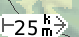
\includegraphics[angle=0,width=0.3\linewidth,keepaspectratio='true']{figures/zoom.png}}  Die Zahl gibt hierbei die Gesamtbreite des Bildschirmes an.

Für \textsc{Compaq Aero} Benutzer: Wenn Ihr die \textsl{Compaq Aero Game Keys} aktiviert (im Q-Menü), können auch diese für das Hinein- und Herauszoomen benutzt werden.\index{Zoom!Maßstab}

\subsection*{Steigflug Zoom}\index{Zoom!Steigflug}
Es besteht die Möglichkeit, zwei Zoom Einstellung zu haben: einer, wenn der Segelflieger beim Kurbeln ist, und ein weiterer welcher für den Überlandflug bzw. Endanflugmodus gültig ist.

Dies ist die ''Steigflug Zoom'' Einstellung, welche unter \config{circlingzoom} eingestellt werden kann.\index{Zoom!Steigflug}

Als Standardmaßstab für die ''Steigflug Zoom'' Einstellung ist abhängig  von der Displaygröße ein Kartenmaßstab von 2,5 - 5 km voreingestellt.
Wenn während des Kurbelns hinein oder herausgesucht wird, so beeinflußt dies nicht den vorher im Grabe Ausflug eingestellten zu den Zoom-Maßstab. Sowie das kurbeln beendet wird, wird automatisch auf den vorher eingestellten Maßstab zurückgesetzt.
\subsection*{Auto Zoom}\label{sec:AutoZoom}\index{Zoom!Auto}
Die ''Auto-Zoom'' Funktion zoomt automatisch herein, wenn man sich einem Wendepunkt nähert.\index{Zoom!Auto}
\menulabel{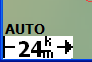
\includegraphics[angle=0,width=0.35\linewidth,keepaspectratio='true']{figures/zoomauto.png}}
Wenn Auto-Zoom aktiv ist, erscheint und links unten am Kartenrand der Text ''Auto-Zoom'' über dem derzeitigen Kartenmaßstab.
Es kann trotzdem weiterhin hinein und heraus gesucht werden, die Auto-Zoom Funktion wird in diesem Falle automatisch auf manuell zurückgesetzt.

Um Auto-Zoom einzuschalten, benutze links angegebenes Menü
%\begin{quote}
%\smenus{Anzeige}\blink\smenut{Zoom}{Auto}
%\end{quote}
\menulabel{\bmenut{Anzeige}{1/2}\blink\bmenut{Zoom}{Auto}}
Nachdem sich ein Wegpunkt geändert hat (sei es automatisch, über die Wegpunkt Auswahl, oder durch manuelles Umschalten auf der Karte) wird ''Auto-Zoom'' den Maßstab automatisch so wählen, daß der nächste Wegpunkt sichtbar ist. Während des Kurbelns wird die Karte zentriert bezüglich des Bartes dargestellt, sodaß das Flugzeugsymbol dennoch sichtbar bleibt.

%%%%%%%%%%%%%%%%%%%%%%%%%%%%%%%%%
\section{Verschieben der Karte - Verschiebe-Modus}\index{Karte!Verschieben}\index{Pan-Mode}

Der Verschiebe-Modus (''Pan-Mode'') erlaubt es dem Benutzer die Karte auf der moving map zu verschieben. Damit ist er in der Lage einen weit größeren Bereich zu sehen als auf den Kartenausschnitt dargestellt wird. Insbesondere bei der Aufgabenplanung ist dies sinnvoll und nützlich.


\menulabel{\bmenut{Anzeige}{1/2}\blink\bmenut{Verschieben}{Ein}}

%\begin{enumerate}
%\item Einschalten des Verschiebe-Modus wie folgt:
%\begin{quote}
%\smenus{Anzeige}\blink\smenut{Verschieben}{Ein}
%\end{quote}
 
Die Karte kann nun mit auf den Touchscreen gedrückten Finger verschoben werden. Auf dem \textsf{PC}  erfolgt dies mit der Maus bei gedrückt gehaltener Maustaste; beim \al werden der innere und äußere Drehknopf hierzu benutzt. Der Verschiebemodus wird verlassen mit 
%\menulabel{\bmenut{Verschieben}{Aus}} 
\button{Verschieben Aus}
%\begin{quote}
%\smenut{Verschieben}{Aus}
%\end{quote}
%\end{enumerate}

Es erscheint ein spezielles Verschiebe-Menü (s.u.) sowie ein Fadenkreuz, welches immer in der Mitte der Karte fixiert bleibt.

Der Verschiebe-Modus kann ebenso über die Geste P \gesture{P} aufgerufen werden. Weiterhin ist es möglich mit der bei Apple und Android üblichen Geste 
für vergrößern oder verkleinern (Finger spreizen oder zusammenziehen) in den Verschieben-Modus  zu kommen.

\begin{center}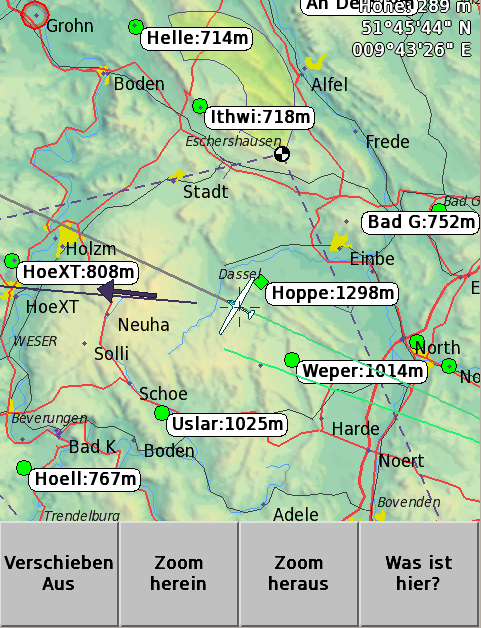
\includegraphics[angle=0,width=0.75\linewidth,keepaspectratio='true']{figures/pan.png}
\end{center}\index{Was ist hier?}
Mit der Auswahl von \button{Was ist hier} öffnet sich ein Menü, welches entsprechende Kartenelemente wie z.B.\ Wegpunkte und Lufträume die sich in der Nähe des Fadenkreuzes befinden, sowie die eigene Position anzeigt und zur Auswahl/Bearbeitung darstellt. Zu den jeweiligen angezeigten Elementen werden Entfernung und ggf.\ benötigte Höhe angezeigt.

Parallel dazu werden in der oberen rechten Bildschirmecke die Koordinaten des Fadenkreuzes und die dazugehörige Höhe des Geländes über MSL angegeben.  

%%%%%%%%%%%%%%%%%%%%%%%%%%%%%%%%%%%
\section{Wegpunkte} \label{sec:waypoint-schemes}
Die Darstellung und Einfärbung von Wegpunkten erfolgt je nach Situation und Art des jeweiligen Punktes.\menulabel{\bmenut{Konf}{2/3}\blink\bmenus{System}} Hauptmerkmal ist die hierbei Landbarkeit bzw. Erreichbarkeit eines Wegpunktes.

Es gibt derzeit drei verschiedene Icon- Sätze  für die Darstellung von landbaren Wegpunkten  (Lila Punkt, Schwarz Weiß und Ampel), die unter \index{Wegpunkte!Farben}
%\begin{quote}
%\smenus{Konfig.}\blink\smenus{Konfig.}\blink\smenut{System}%{Einstellung}\blink\seite{4}
%\end{quote}
\button{Landbare Symbole} ausgewählt werden können.\menulabel{\button{Kartenanzeige}\blink\button{Wegpunkt}}\index{Wegpunkte!Darstellung}

\begin{description}
   \item[\p{Lila Punkt}] Bei dieser Darstellung werden die landbaren Plätze als lila Punkt angezeigt. Wenn der Wegpunkt erreichbar ist, bekommt der lila Punkt einen grünen Kreis.  Diese Darstellung ist sehr ähnlich der in WinPilot
   \item[\p{S/W}] \config{waypointicons} Landbare Wegpunkte werden in der Karte weiß/grau dargestellt, ähnlich wie oben bekommen erreichbare Plätze einen grünen Punkt, ist er durch einen Berg versperrt, wird er rot. 
   \item[\p{Verkehrsampel}] Flugplätze und Außenlandefelder werden in den Farben einer Verkehrsampel dargestellt: Grün, wenn erreichbar, Orange, wenn z.B.\ durch einen Berg versperrt und rot, wenn er überhaupt nicht erreicht werden kann.
\end{description}

\tip Je nach verwendeter Datenbank kann auch die Länge und Richtung der Landebahn mit angezeigt werden. 
Weiterhin können je nach Sichtbarkeit bzw. Erreichbarkeit die Farben und/oder Formen geändert werden.

Die Symbole sind in untenstehender Tabelle aufgelistet. 

\begin{tabular}{c|c|cc|ccc|} 
\textbf{Darstellung:} &\begin{sideways}Einfacher Wegpunkt \end{sideways}
&\begin{sideways}WP landbar,  n.  erreichbar\end{sideways}
&\begin{sideways}WP erreichbar\end{sideways}
&\begin{sideways}Flugplatz n. erreichbar\end{sideways}
&\begin{sideways}Flugplatz erreichbar\end{sideways}
&\begin{sideways}Flugplatz versperrt\end{sideways}\\
\hline
''Lila Kreis'' &
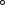
\includegraphics[width=0.5cm]{icons/map_turnpoint.pdf} &

\includegraphics[width=0.85cm]{icons/winpilot_landable.pdf} &

\includegraphics[width=0.85cm]{icons/winpilot_reachable.pdf} &
\rule[0em]{0em}{2.5em}\colorbox{white}{
\includegraphics[width=0.85cm]{icons/winpilot_landable.pdf}}
& 
\includegraphics[width=0.85cm]{icons/winpilot_reachable.pdf} 
& 
\includegraphics[width=0.85cm]{icons/winpilot_marginal.pdf} \\
\hline
''Schwarz/Weiß''  &
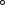
\includegraphics[width=0.5cm]{icons/map_turnpoint.pdf} &

\includegraphics[width=0.75cm]{icons/alt_landable_field.pdf} &

\includegraphics[width=0.75cm]{icons/alt_reachable_field.pdf} &
\rule[0em]{0em}{2.5em}\colorbox[rgb]{0.94,0.94,0.94}{
\includegraphics[width=0.75cm]{icons/alt_landable_airport.pdf}}
& 
\includegraphics[width=0.75cm]{icons/alt_reachable_airport.pdf} 
& 
\includegraphics[width=0.75cm]{icons/alt2_landable_field.pdf}\\
\hline
''Verkehrsampel'' &
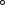
\includegraphics[width=0.5cm]{icons/map_turnpoint.pdf} &

\includegraphics[width=0.75cm]{icons/alt2_landable_field.pdf} &

\includegraphics[width=0.75cm]{icons/alt_reachable_field.pdf} &
\rule[0em]{0em}{2.5em}\colorbox{white}{
\includegraphics[width=0.75cm]{icons/alt2_landable_airport.pdf}}
&
\includegraphics[width=0.75cm]{icons/alt_reachable_airport.pdf} 
&
\includegraphics[width=0.75cm]{icons/alt2_marginal_airport.pdf}\\
\hline
\end{tabular}
%
 
Die Wegpunkte können nach mehreren Abkürzungsregeln beschriftet werden, um auf \config{labels}
\menulabel{\bmenut{Anzeige}{2/3}\blink\bmenut{Beschriftung}{Aufgabe}} der Karte nicht so viel Platz zu verschwenden und den Bildschirm  übersichtlicher darstellen zu können. 
So können die Beschriftung der Wegpunkte nur für die Aufgabe, für Aufgabe und Landeplätze oder aber für alle Wegpunkte aktiviert weren.


\xc berechnet kontinierlich und unter Berücksichtigung des Windes, welche Wegpunkte sich innerhalb des Gleitpfades befinden und stellt dies entsprechend der eingestellten Optionen dar.

Die angenommene Ankunftshöhe {\em oberhalb der Sicherheitshöhe} der erreichbaren  Wegpunkte wird neben dem Wegpunkt  angezeigt. Diese Ankunftshöhe wird berechnet aus der entsprechenden Leistung des Segelflugzeuges und dem MacCready Wert. 

\config{reachpolar} Hierbei kann gewählt werden, ob die Berechnung mit einem Sicherheits-MacCready Wert, oder aber streng nach der Polare erfolgt.

\subsection*{Nicht landbare Wegpunkte}
Wenn in der  Wegpunktdatenbank bzw. in der Beschreibung des einzelnen Wegpunktes informatiuonen zu dessen beschaffen heit angegeben sind, so werden diese von \xc   entsprechend dargestellt. In der folgenden Tabelle  sind die nicht landbaren Wegpunkte aufgelistet. 

\vspace{9em}
\begin{center}
\begin{small}
\begin{tabular}{ccccccccc}
\begin{rotate}{60}Einfacher Wegpunkt\end{rotate} &
\begin{rotate}{60}Berggipfel\end{rotate} &
\begin{rotate}{60}Aussicht\end{rotate} &
\begin{rotate}{60}Berg-Pass\end{rotate} &
\begin{rotate}{60}Kraftwerk\end{rotate} &
\begin{rotate}{60}Turm/hohes Gebäude\end{rotate} &
\begin{rotate}{60}Tunnel\end{rotate} &
\begin{rotate}{60}Wetterstation\end{rotate} &
\begin{rotate}{60}Brücke\end{rotate}\\
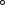
\includegraphics[width=0.5cm]{icons/map_turnpoint.pdf} &
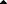
\includegraphics[width=0.8cm]{icons/map_mountain_top.pdf} &
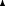
\includegraphics[width=0.7cm]{icons/map_obstacle.pdf} &
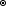
\includegraphics[width=0.7cm]{icons/map_pass.pdf} &
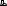
\includegraphics[width=0.8cm]{icons/map_power_plant.pdf} &
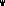
\includegraphics[width=0.7cm]{icons/map_tower.pdf} &
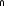
\includegraphics[width=0.6cm]{icons/map_tunnel.pdf} &
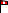
\includegraphics[width=0.6cm]{icons/map_weather_station.pdf} &
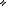
\includegraphics[width=0.8cm]{icons/map_bridge.pdf} \\
\end{tabular}
\end{small}
\end{center}


%%%%%%%%%%%%%%%%%%%%%%%%%%%%%%5
\section{Aktive Aufgabe}

Die Kurslinie der aktiven Aufgabe wird als eine grüne, gestrichelte Linie auf der Karte dargestellt.

Bei AAT-Aufgaben werden die Sektoren der Aufgabe gelb transparent hinterlegt dargestellt.
Die Start und Zielpunkte werden als Kreise dargestellt, Linien werden nur 
gezeichnet, wenn es sich hierbei um Start bzw. Ziellinien handelt.
Wendepunktsektoren werden als Segmente dargestellt (auch der DAEC-Schlüssellochsektor kann dargestellt werden).


Vom Segelflugzeugsymbol wird eine dicke schwarze Linie direkt zum nächsten aktiven Wendepunkt gezeichnet. Diese Linie stellt normalerweise den direkten Weg zum nächsten Wegpunkt dar, kann aber auch eine {\em Route} darstellen, welche um zum Beispiel Berge und/oder Lufträume herum führt. Nähere Details hierzu werden im Abschnitt Route~\ref{sec:route}  beschrieben.
\begin{center}
\begin{tabular}{c c c}
{\it Start/Ziel} & {\it Sektor} & {\it Zylinder} \\
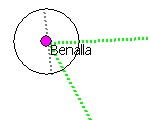
\includegraphics[angle=0,width=0.3\linewidth,keepaspectratio='true']{figures/cut-startfinish.png} &
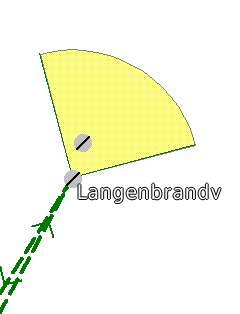
\includegraphics[angle=0,width=0.3\linewidth,keepaspectratio='true']{figures/cut-sector.png} &
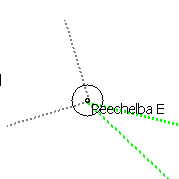
\includegraphics[angle=0,width=0.3\linewidth,keepaspectratio='true']{figures/cut-barrel.png} \\
\end{tabular}
\end{center}
%%%%%%%%%%%%%%%%%%%%%%%%%55
\section{Gelände und Topologie}

Die folgenden topologischen Details werden auf der Karte dargestellt:
\begin{itemize}
\item Hauptstraße, dargestellt als rote Linien
\item Flüsse, dargestellt als blaue Linien
\item Große Wasserflächen (Seen), dargestellt als blaue Flächen
\item Große Städte, dargestellt als gelbe Flächen
\item Kleine Siedlungen, dargestellt als gelbe Diamanten, je nach verwendeter Datenbank wird auch nur der Name angezeigt 
\end{itemize}
Großstädte und kleine Siedlungen werden in Schrägschrift beschriftet.

Das Gelände wird gemäß der Höhe eingefärbt, optional kann es schattiert werden -  entweder gemäß der Sonneneinstrahlung oder aber entsprechend des Windeinfalles (Luv oder Lee).

Unbekanntes Gelände, oder Gelände das unterhalb der Meereshöhe liegt, wird blau dargestellt.

Die Schattierung des Geländes erhöht die Erkennbarkeit der Struktur und ist derzeit so gestaltet, daß helle Flächen eines Berges die Luvseite darstellen \config{shading}. und dunkle Flächen die Leeseite.
Die Stärke und Helligkeit der Schattierung kann konfiguriert werden 

Die Unterstützung der Schattierung für Sonneneinstrahlung in Abhängigkeit vom \menulabel{\bmenut{Anzeige}{2/2}\blink\bmenut{Gelände}{An}}Sonnenstand ist in Arbeit\dots.
Gelände- und Topologiedarstellung kann über das Menü ein und ausgeschaltet werden:
%\begin{quote}
%\smenus{Anzeige}\blink\smenus{Anzeige}\blink\smenut{Gelände}{An} \\[1em]
%\smenus{Anzeige}\blink\smenus{Anzeige}\blink\smenut{Topologie}{An}
%\end{quote}

\menulabel{\bmenut{Anzeige}{2/2}\blink\bmenut{Topologie}{An}}
\begin{center}
\begin{tabular}{c c}
Topology & Terrain \\
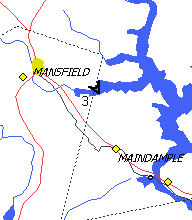
\includegraphics[angle=0,width=0.4\linewidth,keepaspectratio='true']{figures/cut-topo.png} &
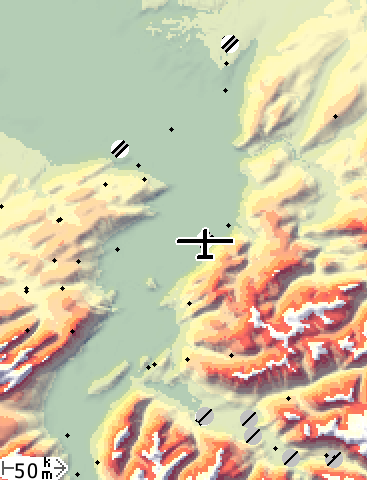
\includegraphics[angle=0,width=0.4\linewidth,keepaspectratio='true']{figures/cut-terrain.png} \\
\end{tabular}
\end{center}

Wenn keine Geländedaten zur Verfügung stehen (oder die Gelände-Anzeige ist abgeschaltet) erscheint der Hintergrund der Karte weiß. Jedes Gelände unterhalb des Meeresspiegels wird blau dargestellt!
Flüge außerhalb des in der Datenbank bekannten Geländes werden weiß dargestellt.

\menulabel{\bmenut{Anzeige}{2/2}\blink\bmenut{Beschriftung}{Alle}}
Um die Darstellung auf der Karte übersichtlicher zu machen, können Beschriftungen und Labels der Wegpunkte ein und ausgeschaltet werden, oder aber auf die aktive Aufgabe beschränkt werden.


%\begin{quote}
%\begin{center}
%\smenus{Anzeige}\blink\smenus{Anzeige}\blink\smenut{Beschriftung}%{Keine}\blink\smenut{Beschriftung} {Aufgabe}\blink \dots
 %\\[0.75em] \smenut{Beschriftung}{Alle}\blink\bmenud{Beschriftungen}{Aufgabe\&}
%{Landeplätze}
%\end{center}
%\end{quote}

Folgende Auswahlen stehen zur Verfügung:

\jindent{\bmenud{Beschriftungen}{Aufgabe \&}{ Landeplätze}}{ Zeigt die Beschriftung der Wegpunkte  der aktiven Aufgabe und einige landbare Felder (basierend auf den Wegpunkt-Details in der geladenen Wegpunkt Datei).  Andere Wegpunkte werden angezeigt, aber nicht beschriftet. }
\jindent{\bmenut{Beschriftung}{Aufgabe}}{ Es werden nur die in der aktiven Aufgabe befindlichen Wegpunkte beschriftet. }
\jindent{\bmenut{Beschriftung}{Alle}}{ Anzeige aller Beschriftungen für alle Wegpunkte. }

Die Beschriftung und das Aussehen der Beschriftung ist über das Menü \config{labels} konfigurierbar.
%%%%%%%%%%%%%%%%%%%%%%55
\section{Flugspur (trail)}\label{sec:trail}

Wenn gewünscht, kann die bisher geflogen Flugstrecke auf der Karte dargestellt werden. Die Farbe und die Breite dieser Spur hängt von der Höhe oder von Vario-Wert ab und kann entsprechend gewählt werden. \config{snailtype}

\begin{center}
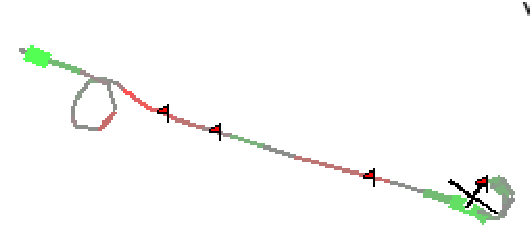
\includegraphics[angle=0,width=0.75\linewidth,keepaspectratio='true']{figures/snail.pdf}
\end{center}

Wenn ein VEGA-Variometer angeschlossen ist und die Netto-Luftmassenbewegung anzeigt, dann können die Farben und Dicken dieser Spur auch die Netto-Luftmassenbewegung darstellen.

Die Flugspur kann wie folgt ausgewählt werden: \button{Kurz} (zeigt ungefähr 10 min), \menulabel{\bmenut{Anzeige}{2/2}\blink\bmenut{Spur}{Kurz}} \button{Lang}, (zeigt ca. eine Stunde), \button{Voll} (zeigt die gesamte bisherige Flugstrecke) und aus. Die Einstellung kann jederzeit über das Menü wie folgt vorgenommen werden:

%\begin{quote}
%\smenus{Anzeige}\blink\smenus{Anzeige}\blink\smenut{Flugspur}%{Lang}\blink\smenut{Flugspur}{ Kurz}
%\end{quote}

Alternativ kann die Einstellung auch im Menü  \config{snailtrail} als Voreinstellung eingestellt werden.
Beachtet, daß wegen der Übersichtlichkeit der Kartendarstellung beim Kurbeln die Flugspur grundsätzlich kurz ist.
%%%%%%%%%%%%%%%%%%%%%%%%%%%%%%
\subsection*{Spurdrift (Windversatz-Kompensation)}
Um den Windversatz beim Kurbeln darzustellen und so das Zentrieren zu unterstützen, kann die Spurdrift-Funktion bei der Kartendarstellung eingeschaltet werden.

 \textcolor{blue}{ Die Spurdrift bzw. Windversatz-Kompensation nach Kap.\ref{sec:Windeinstellung} hat \textbf{nichts}  mit der Funktion ''geschätzte Windabdrift'' \achtung aus der Endanflugskonfiguration nach Kap.~\ref{sec:final-glide} zu tun!}
 
In diesem Fall wird die Flugspur relativ zum Wind aufgezeichnet und nicht mehr absolut über Grund. Das bedeutet, daß  \xc den erflogenen Bart während des Fluges mit dem ermittelten Wind versetzt ganz ähnlich wie auch das Flugzeug versetzt wird. Hiermit wird eine bessere Wiederauffindbarkeit und  Anzeige der Bewegung des Flugzeuges relativ zum Bart ermöglicht.

Zur Veranschaulichung ist nachfolgend ein Beispiel beigefügt. 

Beachte, daß, wenn die Spurdriftfunktion aktiviert ist (rechtes Bild), sich das Flugzeug mehr in einem parallelversetzten Kreis  bewegt, anstelle einer gekrümmten, langgezogenen Spirale (linkes Bild).

\begin{center}
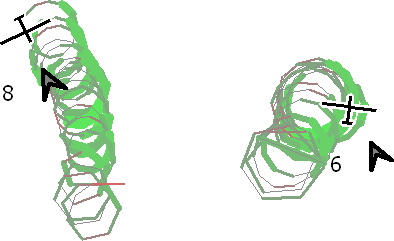
\includegraphics[angle=0,width=0.8\linewidth,keepaspectratio='true']{figures/traildrift.png}
\end{center}

\config{traildrift} Die Funktion \button{Spurdrift} kann über die Konfiguration Einstellung ein und ausgeschaltet werden.  Die Kompensation ist ausschließlich in Kurbelmodus aktiv; im normalen Geradeausflug wird eine Kompensation über das Wind-Menü ermöglicht.
\menulabel{\bmenus{Konfig}\blink\bmenus{Wind}}
Die Anzeige des Windversatzes zeigt sehr schön, wenn Bärte in der Höhe stark versetzt werden - zum Beispiel durch Windscherungen.

Die Breite der Flugspur  kann optional anhand des Vario-Wertes gesetzt werden (Steigen, Saufen) \config{trailscaled}.
%%%%%%%%%%%%%%%%%%%%%%%5
\section{Marker}

Marker werden als kleine blaue Flaggen auf der Karte dargestellt. 
Die Marker können entweder automatisch oder aber durch Knopfdruck gesetzt werden.

\menulabel{\bmenut{Nav}{2/2}\blink\bmenut{Marke}{Setzen}}Ein Beispiel für die Nutzung von automatischem Setzen von Markern ist z.B. die 
Markierung, wann in den Kurbelmodus gewechselt wurde. Hiermit kann sehr einfach dargestellt werden, wann und wo gekurbelt wurde.\index{Marker}
\menulabel{
\includegraphics[angle=0,width=0.5cm,keepaspectratio='true']{icons/map_flag.pdf}}

Marker werden nicht gespeichert, wenn \xc beendet wird, die Koordinaten aller Marker werden jedoch im File \verb|xcsoar-marks.txt| gespeichert.

%%%%%%%%%%%%%%%%%%%%%%%%%%%%%%
\section{Anzeige des Gleitbereiches}\label{sec:reach}

Der aktuelle Gleitbereich \button{Erreichbar Anzeige}kann wahlweise in der Karte auf zwei Weisen dargestellt werden:\index{Gleitbereich}\index{Gleitbereich!Darstellung}\index{Reichweite}
\menulabel{\bmenut{Konfig.}{2/3}\blink\bmenus{System}}
\begin{itemize}
    \item als schwarz-weiß gestrichelte Linie, 
    \item als schattierter Bereich.
\end{itemize}
\menulabel{\button{Endanflug}\blink\button{Routenplaner}}
Der Gleitbereich schließt alle erreichbaren Gelände ein und markiert - entsprechend der Höhe des Geländes - auch Bereiche, welche evtl.\ umflogen werden müssen.  Dies kann sehr nützlich sein, wenn in niedrigen Höhen nach Steigen gesucht wird, oder man sich in bergigem Gelände aufhält.

Die Berechnung der Reichweite \button{Reichweite Modus} kann in zwei Detailstufen \config{turningreach} wie folgt konfiguriert werden:

\begin{description}
\item[\p{Aus}] Wenn ausgeschaltet, wird die Reichweite nicht berechnet.
\begin{center}
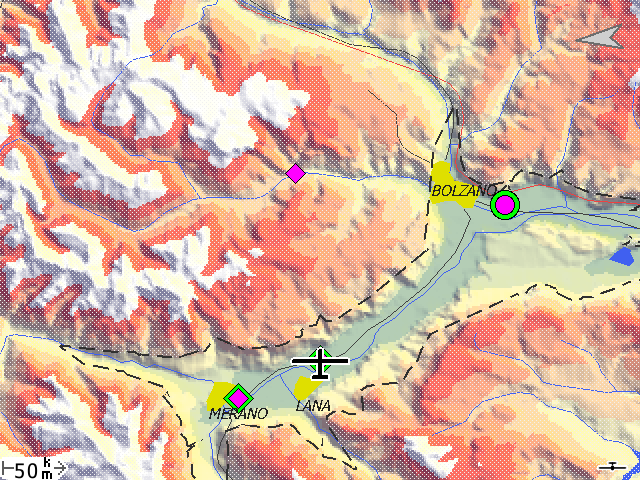
\includegraphics[angle=0,width=0.8\linewidth,keepaspectratio='true']{figures/reach2.png}
\end{center}
\item[\p{Direkt}] Wenn eingeschaltet, erfolgt die Berechnung der Reichweite geradeaus vom Flugzeug. Es werden weder Lufträume noch sonstige Hindernisse in die Kalkulation einbezogen.\index{Gleitbereich!Berechnung}
 \item[\p{mit Umweg}] Wenn dies eingeschaltet ist, wird die Reichweite unter Berücksichtigung von max.\ drei 90$^\circ$ Kurven errechnet, die z.B.\ zum umfliegen von kleineren Hindernissen bzw.\ zum Umschauen benötigt werden. Diese Reichweite ist entsprechend geringer (s.\ Bilder)
\begin{center}
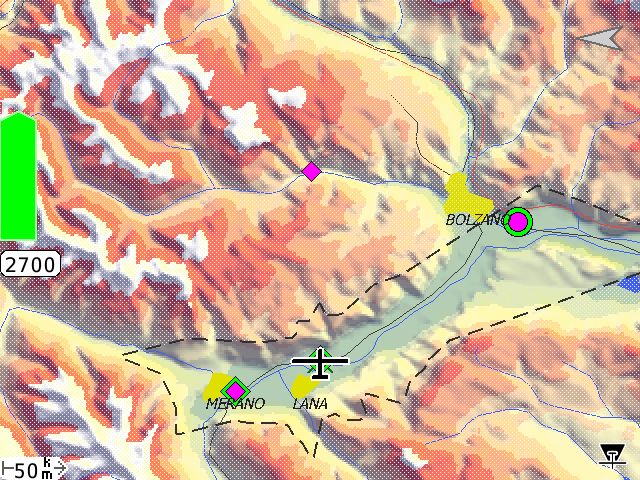
\includegraphics[angle=0,width=0.8\linewidth,keepaspectratio='true']{figures/reach1.png}
\end{center}
\end{description}

Der Weg des Endanfluges wird permanent auf evtl.\ Kollisionen mit einer Geländeerhebung geprüft -- sollte sich eine Kollisionsgefahr ergeben, so wird der vorausgesagte Kollisionspunkt\index{Geländekollision} mit dem Gelände als kleines rotes Kreuz auf der Karte dargestellt.

Wenn der \button{Reichweite Modus} aktiviert ist, dann wird dieser bei Abbruch einer Aufgabe  automatisch benutzt, um landbare Plätze (in allen Richtungen) auf der Karte darzustellen (Im Alternativen - Modus).


\textcolor{blue}{Beachte, daß bei aktiven Aufgaben die ''Reichweite'' Funktion   \textbf{nicht} in den InfoBoxen aktiv ist, hier wird die Funktion \textbf{nicht} verwendet!}\warning 


\textcolor{blue}{Sie ist ausschließlich bei der Darstellung auf der Karte und bei abgebrochenen Aufgaben aktiv!}

Die Leistungsdaten des Segelflugzeuges (Polare) bzw.\ die MacCready Einstellung, die für diese Berechnung verwendet werden sollen, können unter %\ref{sec:final-route}
\button{Erreichbare Polare} eingestellt werden. \config{reachpolar}
\begin{description}
\item[\p{Aufgabe}] Es wird der MC benutzt, welcher in der Aufgabe gesetzt ist.
\item[\p{Sicherheits  MC}] Hier wird ein voreingestellter, i.d.R.\ niedriger MC Wert gewählt, den der Pilot vorher festsetzt. Normalerweise etwas schlechter als das beste Gleiten. (s.~\ref{safety-MC}) 

Die ''Größe'' der Sicherheit bei der Reichweitenkalkulation ist dementsprechend   die Differenz aus bestem Gleiten und dem Gleiten entsprechend der Geschwindigkeit des Sicherheits MC-Wertes.
\end{description}
%%%%%%%%%%%%%%%%%%%%%%%%%%%%%%%%%%%%%%%%%5
\section{Status-Fenster}\label{sec:aircr-stat-dial}\index{Status}

Das Status-Fenster ist ein reines Informationsfenster und hat fünf Unterfenster. \button{Flug}, \button{System}, \button{Aufgabe}, \button{Regeln} und \button{Zeiten} Es 
\menulabel{\bmenut{Info}{2/3}\blink\bmenus{Status}} und dient vor allem zur Beobachtung von Zeiten, Koordinaten, Regeln etc.\  
  
\achtung Beachte, daß die hier aufgeführten Daten \textbf{nicht} aktualisiert werden, während dies Fenster geöffnet ist. erst nach Schließen und wieder aufrufen sind die Daten wieder auf dem laufenden! 


%\begin{center}
%\includegraphics[angle=0,width=0.5\linewidth,keepaspectratio='true']{figures/XCS64-StatusWindow.png}
%\end{center}

Mit dem Button \button{Flug} kann z.B. schnell Deine Position an andere 
weitergegeben werden, hier wird Deine Position angezeigt, Deine Peilung und Entfernung auf den nächsten aktiven Wegpunkt etc. 


Derzeit werden als ''nächste Wegpunkte'' ausschließlich Punkte aus der Wegpunkt-Datenbank genommen, in zukünftigen Versionen ist geplant, evtl.\  auch Dörfer und Städte aufzunehmen.%\menulabel{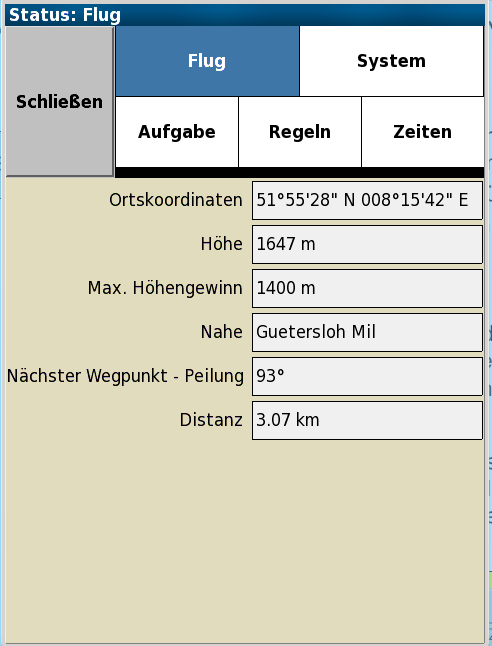
\includegraphics[angle=0,width=0.8\linewidth,keepaspectratio='true']{figures/status-flight.png}}
\sketch{figures/status-flight.png}

Unter \button{Regeln}kannst Du z.B.\ erkennen, ob Dein Abflug gültig war, mit welcher Geschwindigkeit er erfolgte etc.\ 

\button{Zeiten}gibt allerlei Zeiten wieder, z.B.\ die UTC-Zeit, den Sonnenauf- und Untergang (Danke, Helmut\dots), Start- Lande- und Flugzeit. 

\button{System}informiert u.a.\ über die Versorgungsspannung des Geräte, wie der GPS-Empfang ist, ob \fl und Logger angeschlossen sind. 

In \button{Aufgabe}werden Daten und Zeiten zur aktuellen Aufgabe gelistet: aktueller Schnitt, Distanz, bei AAT: zugeteilte und verbleibende Zeit etc\dots 


%%%%%%%%%%%%%%%%%%5
\section{Routen}\label{sec:route}

\xc kann Flugwege planen, die um Lufträume und z.B.\ Gebirge herumführen, sowohl in \menulabel{\bmenut{Konfig.}{2/3}\blink\,\bmenus{System}}
horizontaler als auch in vertikaler Richtung. Solch ein Flugweg wird hier als ''Route'' bezeichnet und kann mit dem \button{Routenplaner} konfiguriert werden..

\menulabel{\qquad\button{Endanflugrechner}} 
Die Höhe des Zieles ist hierbei die Ankunftshöhe des Zieles, kann aber auch größer sein, falls die Wegführung durch die in der Aufgabe deklarierten Wegpunkte dies erfordern. Die Routen-Funktion ist in folgenden Flugmodi verfügbar:

''Gehezu'', deklarierte (aktive) ''Aufgaben'' und ''Abbruch''.

\begin{center}
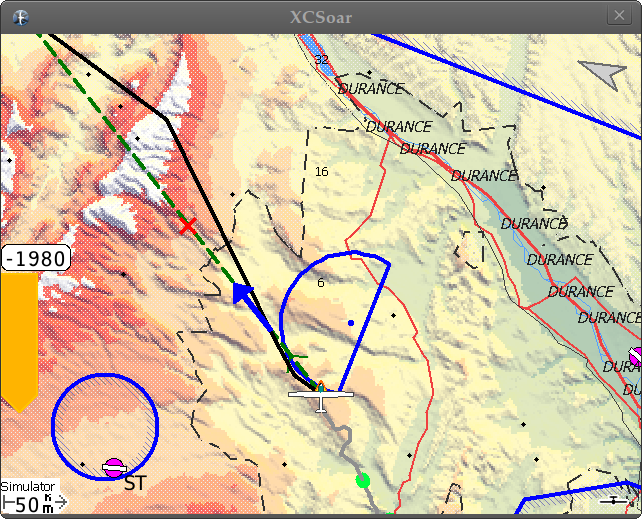
\includegraphics[angle=0,width=0.75\linewidth,keepaspectratio='true']{figures/route3.png}
\end{center}

Im obigen Bild kannst Du gut erkennen, wie die ''Route'' einen Knick nördlich des Harzes macht, um nicht ins Gelände zu ''stürzen'', der normale Kurs ist gestrichelt weiter südlich zu sehen. 

Bei der Routenberechnung wird die Strecke unter Berücksichtgung der Flugzeugpolaren zeitoptimiert berechnet. Standardmäßig ist die Routenfunktion ausgeschaltet. Sie kann aktiviert werden unter  \config{routemode} Berücksichtigung von Lufträumen, Gelände, Wolkenuntergrenze.

Geländekollisionen in vertikaler Richtung werden verhindert durch Einstellung der Gelände-Sicherheitshöhe. \config{safetyterrain} Hierbei ist keine zusätzliche Höhe als Puffer vorgesehen.

Es kann sein, daß manche Routen in einer Ankunft am Ziel höher als erwartet enden. Dies kann zum Beispiel geschehen, wenn der Zielpunkt exakt hinter einem relativ hohen Berg liegt. Zur Vermeidung von horizontalem Einfliegen in einen Luftraum wird mit ein Sicherheitsabstand von 250 m ohne weitere vertikaler Reserven benutzt.
Richtig deklarierte Routen werden im Flugverlauf über oder unterhalb Lufträumen und auf jeden Fall um Lufträume herum führen.

\warning
Wenn der MacCready-Wert größer als 0, dann ist für den Rechner das Steigen während einer Route gemäß der MC-Theorie ''erlaubt''. \config{routeceiling}  Die maximale Höhe des Steigens  ist auf  500 m unterhalb der Wolkenuntergrenze limitiert, kann jedoch in der Konfiguration abgeschaltet werden.

Ein Steigen über die maximal vorgeschriebene Höhe des Start- und Zielpunktes (siehe oben) wird ''bestraft'' mit einer entsprechend schlechteren Steigrate als der aktuell eingestellte MacCready-Wert. 


Einige Einschränkungen und Limitierung bezüglich des Routenplanungssystems sind hier aufgelistet:

\begin{itemize}
\item Wenn Kurbeln notwendig ist, um das Ziel zu erreichen,  wird angenommen, daß das Steigen zu Beginn der Route ist. 

Hintergrund: eine Einstellung von  MacCready gleich 0 bedeutet, daß (streng nach der MC-Theorie) kein Steigen erwartet wird!  Andernfalls würde die Rechenalgorythmen in  die Irre geführt werden!   
\item Strecken mit Steigen im Geradeausflug werden auf einer konstanten Höhe angenommen, gleichbedeutend mit vielen kleinen Steigen verteilt entlang der Strecke
\item Kurven und Schlenker zwischen den einzelnen Streckensegmenten mit Ablagen größer 90$^\circ$ sind erlaubt
\item Fehler des Rechenalgorithmus innerhalb der Route können dazu führen, daß der Anflug in einem direkten Anflug auf das Ziel zurückgeführt wird.
\end{itemize}


\subsection*{Querschnitt des Geländes und Lufträume auf Kurs (''cross-section'', ''xs'')}
\label{cross-section}\index{Gelände- und Luftraumquerschnitt auf Kurs}\index{Cross-Section (XS)}

Seit Version 6.5 kann auf Wunsch  ein Querschnitt der Fin lugrichtung liegenden
\menulabel{\bmenut{2/3}{Konf.}\blink\bmenus{System}} Lufträume sowie des Geländes
dargestellt werden. Hier sind im oberen Bereich alle derzeit verfügbaren InfoBox-Seiten
aufgelistet und es kann aus gewählt werden, was explizit in welchem Bereich des Bildschirmes
 \menulabel{\bmenus{Aussehen}\blink\bmenus{Seiten}} dargestellt werden soll.
 Darunter ist ein Auswahlbereich vorgesehen, in dem folgende
Möglichkeiten zur Auswahl stehen:
 \begin{description}
 \item[\p{Zentral}] Karte, \fl-Radar, Zentrierhilfe
 \item[\p{InfoBoxen}] Alle derzeit vorhandenen InfoBox-Seiten (max. acht Stück !) werden hier
     zur Auswahl dargestellt. Aux 1 .. Aux 8, Endanflug, Auto, beim Kreisen etc\dots
 \item[\p{Unten}] Nichts, Querschnitt
 \end{description}

Mit der Auswahl \button{Zentral}-- \button{\fl-Radar}kann z.b. eine Seite definiert werden,
auf der als zentrales Element das \fl-Radar dargestellt wird, klickt man dazu unter
\button{Unten} den Punkt \button{Querschnitt}an, wird auf dieser Seite im unteren Bereich der
Querschnitt des auf Kurs liegenden Geländes und der Lufträume mit einem entsprechenden
Maßstab und der Höhe, links am Rand als kleiner schwarzer Pfeil dargestellt. Diese
Querschnitts-Darstellung  wird permanent aktualisiert und stellt so einen schönen  vertikalen
Überblick über das voraus liegende Gelände in Verbindung mit den zu erwartenden Lufträumen
dar.

\begin{center}
\hspace{7.5em}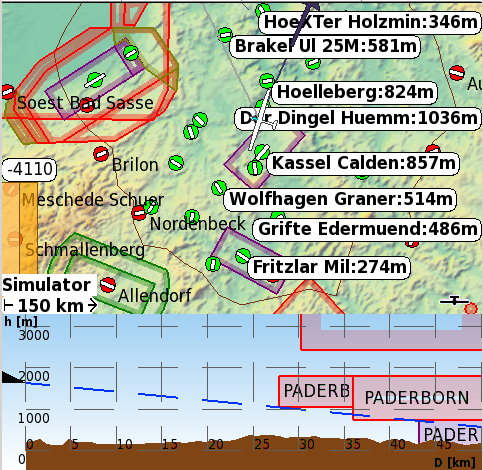
\includegraphics[angle=0,width=0.75\linewidth,keepaspectratio='true']{figures/map-cross-section.png}
\end{center}

Die Querschnitt-Darstellung ist  derzeit nicht skalierbar sondern hat einen fixen horizontalen
Maßstab von 45km und ist auf eine Höhe von 3000m begrenzt.

%Auf diese Art und Weise kann man sich beliebige Infobox-Seiten mit Zusatzinformationen
%erstellen, in welchem z.B.\  beim engen Kurbeln nahe an Lufträumen sehr schön die
%Zentrierhilfe als zentralem Bestandteile der Anzeige und im unteren Bereich der Querschnitt
%über das Gelände dargestellt wird. Diese Seite kann dann als z.B.\ "Kurbeln" bezeichnet und
%abgespeichert werden.

% eben leider nicht  ...  wenn Zentrierhilfe eingeschaltet ist, erscheint cross section nicht.
% bug oder feature ??

Mit den Hoch- und Runterpfeilen kann die Priorität bzw.\ Reihenfolge des Aufrufes der Seiten
auf dem Bildschirm bestimmt werden.  Es ist somit jedem selbst überlassen, wie er sich diese
Anzeigen zurechtlegt.

Mit \button{Hinzufügen} kann eine neue InfoBoxSeite hinzugefügt werden, bis die maximale
Anzahl von 8 Stück erreicht ist.

Mit dem Pfeil nach rechts gelangt man sofort in das InfoBox-Seiten Menü, auf welchem die
einzelnen InfoBoxen innerhalb der Seite definiert und angeordnet  werden können.Die

 \subsection*{\textcolor{blue}{\textbf{{\large Einschränkungen der
Querschnittsdarstellung:}}}}

Die Querschnittfunktion funktioniert derzeit \textbf{nicht} in Verbindung mit der Zentrierhilfe als zentralem Kartenausschnitt!

Die Querschnittfunktion funktioniert derzeit \textbf{nicht} in Verbindung mit dem \fl-Radar als zentralem 
Kartenausschnitt!

\warning {\textbf{Aufgrund technischer
Probleme mit den diversen Betriebsystemen (insbesondere Windows und PPC / Mobile) ist es
derzeit nicht möglich, die Gesten \emph{innerhalb} dieser Area des Bildschirmes beginnen bzw.
Enden zu lassen.}} 

Wenn mit Gesten gearbeitet werden soll, müssen diese daher außerhalb des
Anzeigebereiches des Querschnittes beginnen und enden!

Dies kann zu ungewohnter Arbeitsweise im Fluge führen, da ansonsten die Gesten nicht
ordnungsgemäß ausgeführt werden! Besonders betroffen sind davon Gesten, welche unten
beginnen - diese müssen dann ein Stück weiter oben begonnen werden !!

%finished für v6.5 date 16/02/2013 OH
